\documentclass{beamer}

% choose theme (warning, to use the UniBern theme you need to copy the files beamerthemeUniBern.sty and ublogo.pdf in the same directory)
\usetheme{UniBern}

% packages

\usepackage{graphicx}
\usepackage{hyperref} % allows clickable urls
\usepackage{tikz}
\usepackage{listings} % show code
\usepackage{dsfont} % show code
\usepackage{fontawesome}

% slide numbering
\setbeamertemplate{sidebar right}{}
\setbeamertemplate{footline}{%
	\hfill\usebeamertemplate***{navigation symbols}
	\hspace{1cm}\insertframenumber{}/\inserttotalframenumber}

% define title page
\title{Bayesian workflow for disease transmission modeling in Stan}
\subtitle{{\small Eustat -- XXXIII International Statistical Seminar} }
\author{Julien Riou, MD PhD}
\date{Institute of Social and Preventive Medicine, University of Bern, Switzerland}
\institute{institute}


% begin document
\begin{document}

\frame{\titlepage}

\frame{
	\frametitle{Preface}
	\begin{itemize}
		\item Objective: fit transmission models in Stan 
		\item Based on Grinsztajn et al., 2020 (\underline{\href{https://arxiv.org/abs/2006.02985}{link}})
		\item Prerequisites:
			\begin{itemize}
				\item general understanding of Bayesian inference
				\item basic programming with \texttt{R} and \texttt{Stan}
			\end{itemize}
		\item All material is available on \url{https://github.com/jriou/bayesian_workflow}
	\end{itemize}
}

\frame{
	\frametitle{Outline}
	\begin{itemize}
		\item \textbf{Introduction}
		\item (Quick notice: Bayesian inference with Stan)
		\item Fitting a simple SIR
		\item Simulations to understand the model
		\item Scaling up ODE-based models
		\item Extensions 
	\end{itemize}
}

\frame{
	\frametitle{Introduction}
	Models of disease transmission:
	\begin{itemize}
		\item Interpretability: \alert{mechanistic}, phenomenological
		\item Scale: agent-based, \alert{population-based}
		\item Framework: \alert{deterministic}, stochastic
		\item Data-generating mechanisms: incubation, contagion, immunity...
	\end{itemize}
	\pause
	
	\vspace{2em}
	Mechanistic + population-based + deterministic 
	
	\vspace{1em} $\rightarrow$ \alert{ordinary differential equations (ODE)-based compartmental model} 
}

\frame{
	\frametitle{Introduction}
	ODE-based compartmental model:
	\begin{itemize}
		\item Divide the population into homogeneous groups (\alert{compartments})
		\item Define the \alert{flows} between compartments with ODEs
		\item Define initial conditions (at $t_0$)
		\item Solve for the time-dependent volume in each compartment
	\end{itemize}
	\vspace{1em}
	\pause
	
	The \alert{susceptible-infectious-recovered} (SIR) model:
	\begin{figure}
		\centering
		\scalebox{.8}{
		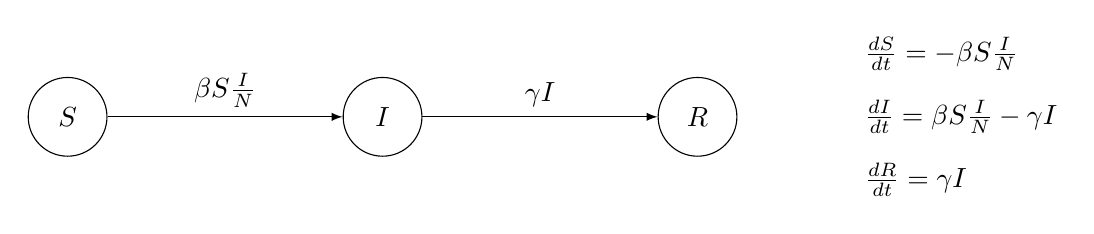
\begin{tikzpicture}
			\node[circle, draw, inner sep=0pt, minimum size=1cm] (S) at (0,0) {$S$};
			\node[circle, draw, inner sep=0pt, minimum size=1cm] (I) at (4,0) {$I$};
			\node[circle, draw, inner sep=0pt, minimum size=1cm] (R) at (8,0) {$R$};
			
			\draw[->,>=latex] (S) edge node[above] { $\beta S \frac{I}{N}$} (I);
			\draw[->,>=latex] (I) edge node[above] { $\gamma I$} (R);
			
			\node[anchor=west] at (10,.8) {$	\frac{dS}{dt} = - \beta S \frac{I}{N}$};
			\node[anchor=west] at (10,0) {$	\frac{dI}{dt} = \beta S \frac{I}{N} - \gamma I $};
			\node[anchor=west] at (10,-.8) {$\frac{dR}{dt} = \gamma I $};
		\end{tikzpicture}
	}
	\end{figure}
}

\frame{
	\frametitle{Introduction}
	
		\begin{figure}
		\centering
		\scalebox{.8}{
			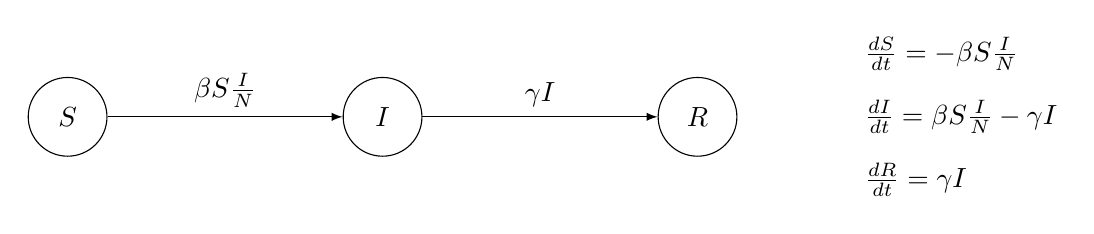
\begin{tikzpicture}
				\node[circle, draw, inner sep=0pt, minimum size=1cm] (S) at (0,0) {$S$};
				\node[circle, draw, inner sep=0pt, minimum size=1cm] (I) at (4,0) {$I$};
				\node[circle, draw, inner sep=0pt, minimum size=1cm] (R) at (8,0) {$R$};
				
				\draw[->,>=latex] (S) edge node[above] { $\beta S \frac{I}{N}$} (I);
				\draw[->,>=latex] (I) edge node[above] { $\gamma I$} (R);
				
				\node[anchor=west] at (10,.8) {$	\frac{dS}{dt} = - \beta S \frac{I}{N}$};
				\node[anchor=west] at (10,0) {$	\frac{dI}{dt} = \beta S \frac{I}{N} - \gamma I $};
				\node[anchor=west] at (10,-.8) {$\frac{dR}{dt} = \gamma I $};
			\end{tikzpicture}
		}
	\end{figure}
	Where:
	\begin{itemize}
		\item $S(t)$ is the number of people \alert{susceptible} to infection
		\item $I(t)$ is the number of people \alert{infected} (i.e. the prevalence)
		\item $R(t)$ is the number of people \alert{recovered} (lifelong immunity)
		\item $N$ is the population size ($S(t)+I(t)+R(t)=N$ for any $t$)
		\item $\beta$ is the \alert{infectious contact rate} (per day per person)
		\item $\gamma$ is the \alert{recovery rate} (1/infectious period)
	\end{itemize}
}

\frame{
	\frametitle{Introduction}
	
	\begin{figure}
		\centering
		\scalebox{.8}{
			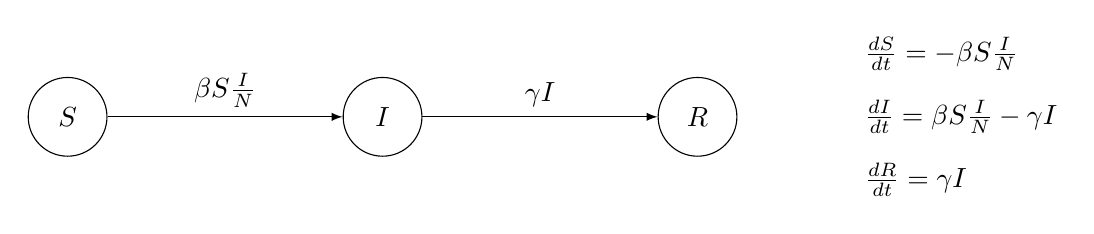
\begin{tikzpicture}
				\node[circle, draw, inner sep=0pt, minimum size=1cm] (S) at (0,0) {$S$};
				\node[circle, draw, inner sep=0pt, minimum size=1cm] (I) at (4,0) {$I$};
				\node[circle, draw, inner sep=0pt, minimum size=1cm] (R) at (8,0) {$R$};
				
				\draw[->,>=latex] (S) edge node[above] { $\beta S \frac{I}{N}$} (I);
				\draw[->,>=latex] (I) edge node[above] { $\gamma I$} (R);
				
				\node[anchor=west] at (10,.8) {$	\frac{dS}{dt} = - \beta S \frac{I}{N}$};
				\node[anchor=west] at (10,0) {$	\frac{dI}{dt} = \beta S \frac{I}{N} - \gamma I $};
				\node[anchor=west] at (10,-.8) {$\frac{dR}{dt} = \gamma I $};
			\end{tikzpicture}
		}
	\end{figure}
	\alert{Intuition} behind the SIR model:
	\begin{itemize}
		\item $I(t)/N$ is the proportion of infected (and infectious)
		\item $\beta I(t)/N$ is the daily number of contacts with infectious people
		\item hence each day, $\beta S I(t)/N$ people become infected (the \alert{force of infection})
	\end{itemize}
}

\frame{
	\frametitle{Introduction}
	
	\begin{figure}
		\centering
		\scalebox{.8}{
			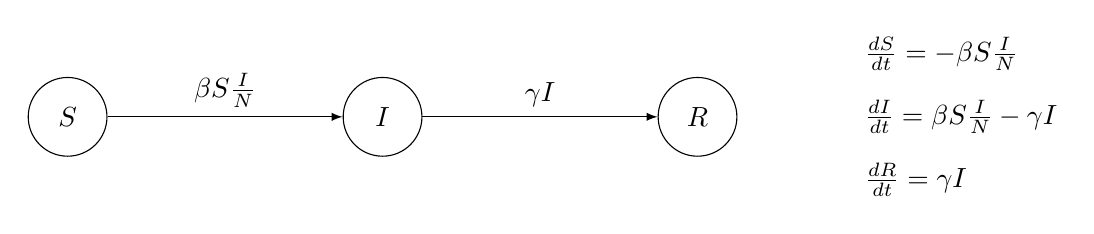
\begin{tikzpicture}
				\node[circle, draw, inner sep=0pt, minimum size=1cm] (S) at (0,0) {$S$};
				\node[circle, draw, inner sep=0pt, minimum size=1cm] (I) at (4,0) {$I$};
				\node[circle, draw, inner sep=0pt, minimum size=1cm] (R) at (8,0) {$R$};
				
				\draw[->,>=latex] (S) edge node[above] { $\beta S \frac{I}{N}$} (I);
				\draw[->,>=latex] (I) edge node[above] { $\gamma I$} (R);
				
				\node[anchor=west] at (10,.8) {$	\frac{dS}{dt} = - \beta S \frac{I}{N}$};
				\node[anchor=west] at (10,0) {$	\frac{dI}{dt} = \beta S \frac{I}{N} - \gamma I $};
				\node[anchor=west] at (10,-.8) {$\frac{dR}{dt} = \gamma I $};
			\end{tikzpicture}
		}
	\end{figure}
	\alert{Assumptions} behind the SIR model:
	\begin{itemize}
		\item homogeneous mixing
		\item $\beta$ and $\gamma$ constant over time
		\item all infections are observed
		\item no incubation, exponentially-distributed recovery
		\item lifelong immunity
		\item stable population
	\end{itemize}
}


\frame{
	\frametitle{Introduction}
	
	Simulate in \texttt{R} with package \texttt{deSolve}:
	
	\begin{itemize}
		\item set compartments and differential equations
	\end{itemize}
	\begin{figure}
		\centering
		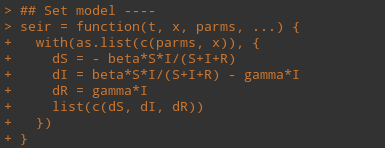
\includegraphics[width=0.55\linewidth]{simple_sir/simsir3.png}
	\end{figure}
	\pause
	\begin{itemize}
		\item set (fixed) values for 		
		$\beta=0.8$; $\rho=1/7$; $S_0=100,000-50$; $I_0=50$ and $R_0=0$
	\end{itemize}
	\begin{figure}
		\centering
		
\includegraphics[width=0.45\linewidth]{simple_sir/simsir1.png}
		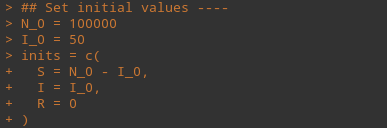
\includegraphics[width=0.45\linewidth]{simple_sir/simsir2.png}
	\end{figure}
}


\frame{
	\frametitle{Introduction}
	\begin{itemize}
		\item solve the ODE system numerically (Runge-Kutta 4th order) to obtain unique solutions for $S(t)$, $I(t)$ and $R(t)$
	\end{itemize}
	$$
f(\beta,\gamma,S_0,I_0,R_0) = \{S(t),I(t),R(t)\}
$$
	\begin{figure}
		\centering
		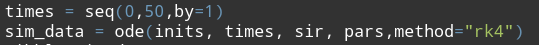
\includegraphics[width=0.65\linewidth]{simple_sir/simsir4.png}
	\end{figure}

}

\frame{
	\frametitle{Introduction}

	\begin{figure}
		\centering
		\only<1>{
			with $\beta=0.8$; $\rho=1/7$; $S_0=100000-50$; $I_0=50$ and $R_0=0$ \\ \bigskip
			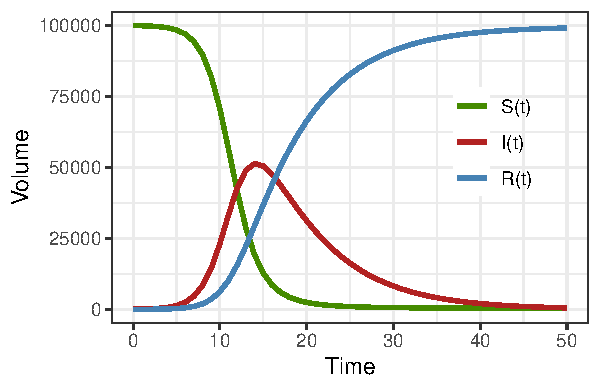
\includegraphics[width=0.7\linewidth]{simple_sir/example_sir1.pdf}
		}
		\only<2>{
			with $\beta = 1.1$ instead of $0.8$, we get \\ \bigskip
			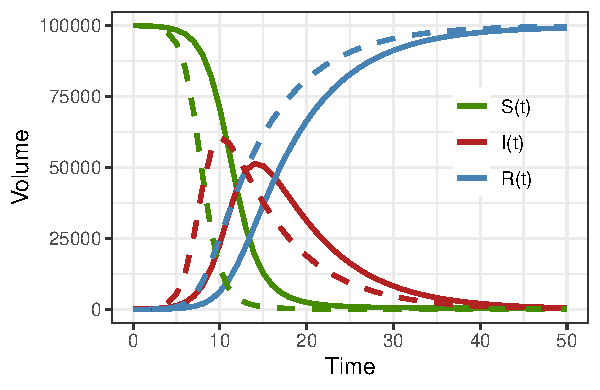
\includegraphics[width=0.7\linewidth]{simple_sir/example_sir2.pdf}
		}
		\only<3>{
			with $\beta = 0.6$ instead of $0.8$, we get \\ \bigskip
			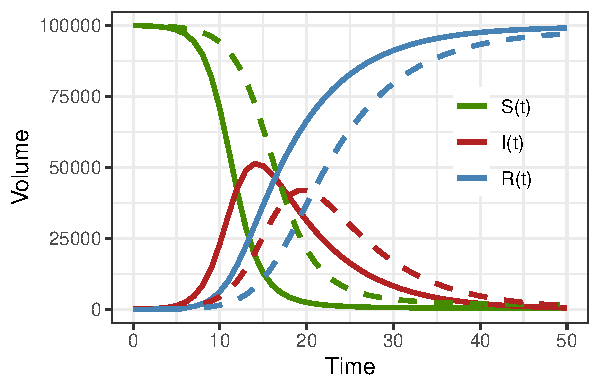
\includegraphics[width=0.7\linewidth]{simple_sir/example_sir3.pdf}
		}
		\only<4>{
		with $\gamma = 1/14$ instead of $1/7$, we get \\ \bigskip
		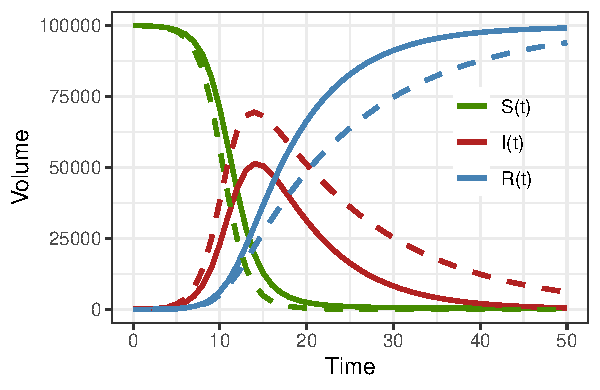
\includegraphics[width=0.7\linewidth]{simple_sir/example_sir4.pdf}
		}
		\only<5>{
		with $\gamma = 1/4$ instead of $1/7$, we get \\ \bigskip
		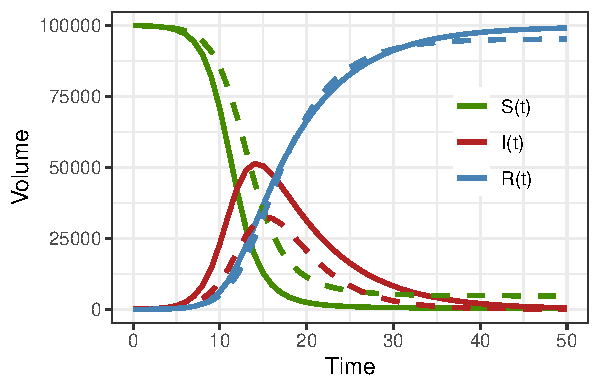
\includegraphics[width=0.7\linewidth]{simple_sir/example_sir5.pdf}
		}
		\only<6>{
		with $I(0) = 500$ instead of $50$, we get \\ \bigskip
		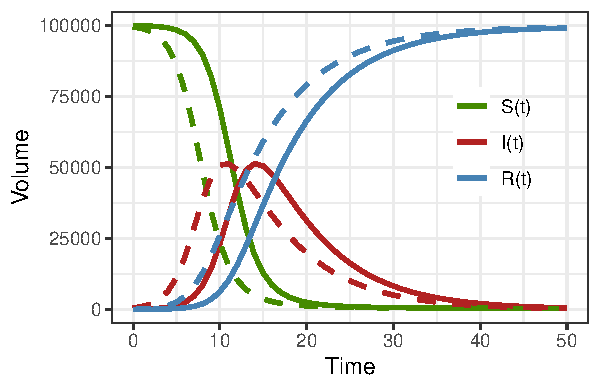
\includegraphics[width=0.7\linewidth]{simple_sir/example_sir6.pdf}
		}
		\only<7>{
		with $I(0) = 5$ instead of $50$, we get \\ \bigskip
		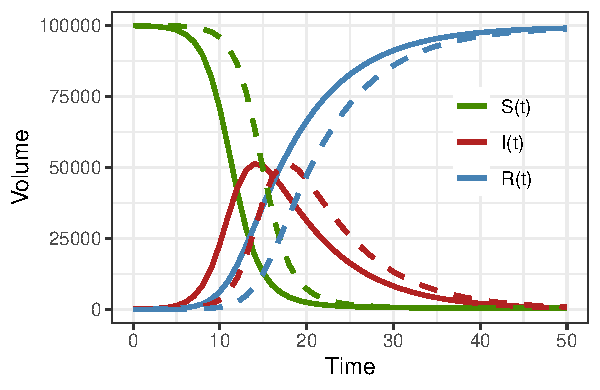
\includegraphics[width=0.7\linewidth]{simple_sir/example_sir7.pdf}
		}
		\only<8>{
		with $R(0) = 20,000$ instead of $0$, we get \\ \bigskip
		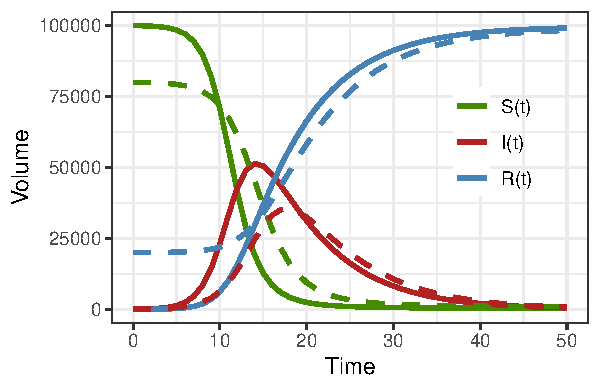
\includegraphics[width=0.7\linewidth]{simple_sir/example_sir8.pdf}
		}
	\end{figure}
}

\frame{
	\frametitle{Introduction}
	Compartmental models have many uses:
	\begin{itemize}
		\item formalize and put numerical values on \alert{general concepts} (herd immunity, vaccination threshold...)
		\item get \alert{mechanistic insight} about an epidemic (transmissibility levels, drivers of transmission)
		$$
		\mathcal{R}_0 = \frac{\beta}{\gamma}
		$$
		
		\item produce precise \alert{forecasts} (based on mechanisms)
	\end{itemize}
	
	\pause\vspace{2em}
	$\rightarrow$ all these uses are based on \alert{numerical values} for $\beta$, $\rho$ and the initial conditions and their \alert{uncertainty}
}

\frame{
	\frametitle{Introduction}
	Enters \alert{Bayesian inference}:
	\begin{itemize}
		\item infer parameter values by \alert{integrating data and domain knowledge}
		\item more efficient for complex models (high dimensionality)
		\item rigorously quantify and propagate uncertainty in parameter estimates and forecast
	\end{itemize}
	
	\pause\vspace{2em}
	$\rightarrow$ Markov Chain Monte Carlo (MCMC) methods and \alert{Stan}
}

\frame{
	\frametitle{Outline}
	\begin{itemize}
		\item Introduction
		\item \textbf{(Quick notice: Bayesian inference with Stan)}
		\item Fitting a simple SIR
		\item Simulations to understand the model
		\item Scaling up ODE-based models
		\item Extensions 
	\end{itemize}
}

\frame{
	\frametitle{(Bayesian inference with Stan)}
	General principle of Bayesian inference:
	\begin{itemize}
		\item specify a complete Bayesian model
		\begin{itemize}
			\item[-] consider data $y = \{y_1,...,y_n\}$ and parameter $\theta$
			\item[-] specify an \alert{observation model} $$\Pr(y|\theta) = \prod_n \text{normal}(y_n | \theta,1)$$
			\item[-] complete the model with a \alert{prior distribution} $$\Pr(\theta) = \text{normal}(0,1)$$
		\end{itemize}
%		\item estimate the \alert{posterior distribution of $\theta$} 
%		$$ \Pr(\theta|y) = \frac{\Pr(y|\theta) \Pr(\theta)}{\Pr(y)}  $$
		\item sample the \alert{posterior distribution} of the parameter
	\end{itemize}
}
%
%\frame{
%	\frametitle{(Bayesian inference with Stan)}
%	The \alert{joint probability density function} of the model is given by
%		$$
%		\Pr(y, \theta)
%		=
%		\prod_{n = 1}^{N} \text{normal\_pdf} \, (y_{n} \mid \theta, 1)
%		\cdot \text{normal\_pdf} \, (\theta \mid 0, 1)
%		$$
%	or on the log scale
%	$$
%	\log \Pr(y, \theta)
%	=
%	\sum_{n = 1}^{N} \text{normal\_lpdf} \, (y_{n} \mid \theta, 1)
%	+ \text{normal\_lpdf} \, (\theta \mid 0, 1) 
%	$$
%}


\frame{
	\frametitle{(Bayesian inference with Stan)}
	Stan is a probabilistic programming framework for Bayesian inference
	\begin{itemize}
		\item it is designed to let the user \alert{focus on modeling} while inference happens under the hood
		\item object-oriented language (based on \texttt{C++}) that supports many  operations, probability densities and ODE solvers
		\item extremely \alert{efficient} MCMC algorithm (Hamiltonian Monte Carlo)
		\item \alert{diagnostic tools} to evaluate the inference
		\item interfaces in \texttt{R} (package \texttt{rstan}), \texttt{python}, \texttt{julia}...	
	\end{itemize}
}



\frame{
	\frametitle{(Bayesian inference with Stan)}
	Programming in Stan is structured in \alert{blocks}:
	\begin{itemize}
		\item the \texttt{data} block defines data variables
		\begin{figure}
			\centering
			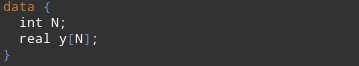
\includegraphics[width=0.6\linewidth]{example_linear/example_linear1.png}
		\end{figure}
		
		\item the \texttt{parameters} block defines parameters
		\begin{figure}
			\centering
			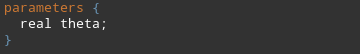
\includegraphics[width=0.6\linewidth]{example_linear/example_linear2.png}
		\end{figure}
		
		\item the \texttt{model} block defines the \alert{target log probability density function}
		\begin{figure}
			\centering
			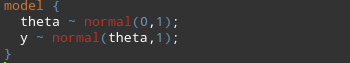
\includegraphics[width=0.6\linewidth]{example_linear/example_linear3.png}
		\end{figure}
		\item save in \texttt{model\_linear.stan}
	
	\end{itemize}
}

\frame{
	\frametitle{(Bayesian inference with Stan)}
	We then explore the target with Stan's MCMC \alert{sampler}:
	\begin{itemize}
		\item load \texttt{rstan} package
		\begin{figure}
			\centering
			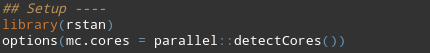
\includegraphics[width=0.7\linewidth]{example_linear/run_stan1.png}
		\end{figure}
		
		\item simulate $N=50$ data points with $\theta=0.7$
		\begin{figure}
			\centering
			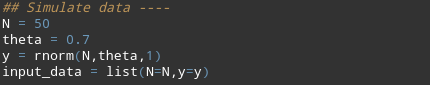
\includegraphics[width=0.7\linewidth]{example_linear/run_stan2.png}
		\end{figure}
		
		\item run MCMC sampling
		\begin{figure}
			\centering
			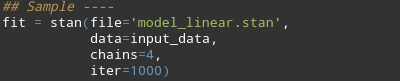
\includegraphics[width=0.7\linewidth]{example_linear/run_stan3.png}
		\end{figure}
	\end{itemize}
}

\frame{
	\frametitle{(Bayesian inference with Stan)}
	We use \alert{multiple chains} that should converge after warm-up
	\begin{figure}
		\centering
		\only<1>{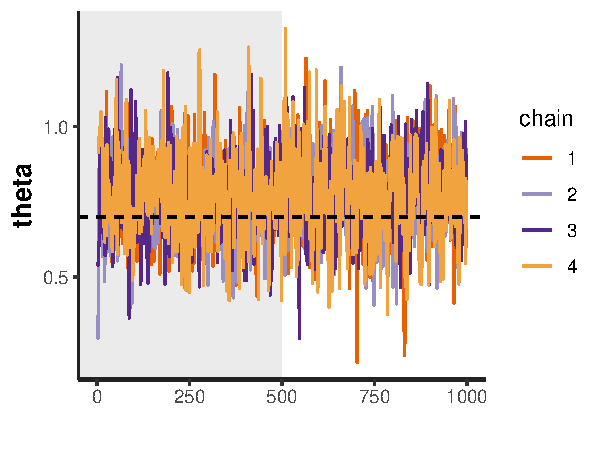
\includegraphics[width=.6\linewidth]{example_linear/trace_theta.pdf}}
		\only<2>{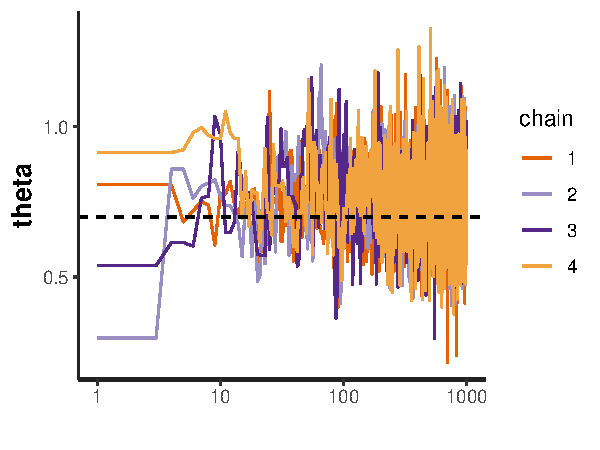
\includegraphics[width=.6\linewidth]{example_linear/trace_theta_init.pdf}}
	\end{figure}
}

\frame{
	\frametitle{(Bayesian inference with Stan)}
	The post-warm-up samples of $\theta$ approximate its \alert{posterior distribution}
	\begin{figure}
		\centering
		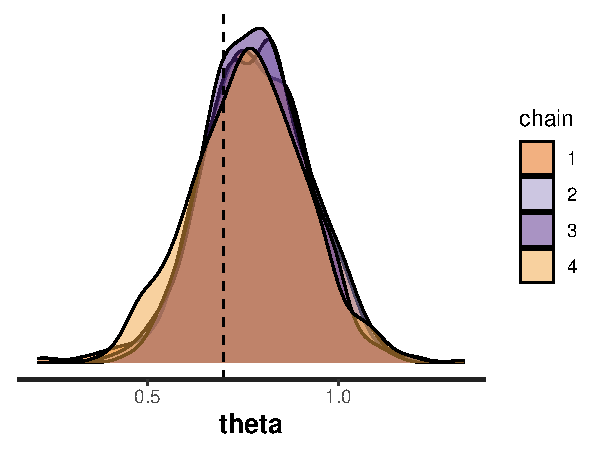
\includegraphics[width=.6\linewidth]{example_linear/post_theta.pdf}
	\end{figure}
}

\frame{
	\frametitle{(Bayesian inference with Stan)}
	
	We run \alert{basic diagnosis tools}: divergences, tree depth, energy
		\begin{figure}
			\centering
			\vspace{1em}
			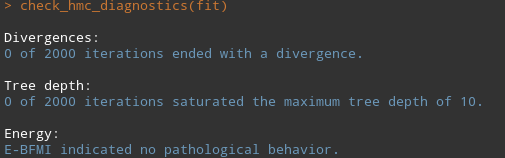
\includegraphics[width=.8\linewidth]{example_linear/run_stan5.png}
		\end{figure}

}

\frame{
	\frametitle{(Bayesian inference with Stan)}
	
	Printing the object gives:
	\begin{itemize}
		\item \alert{diagnostics}: effective sample size, Gelman-Rubin $\hat{R}$
		\item \alert{inference}: full posterior distribution of $\theta$
	\begin{figure}
		\centering
		\vspace{1em}
		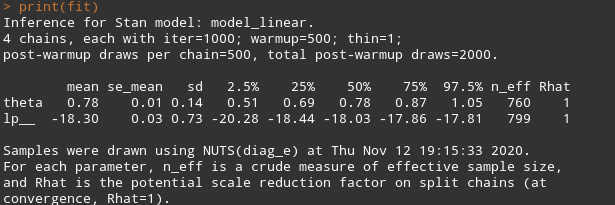
\includegraphics[width=1\linewidth]{example_linear/run_stan4.png}
	\end{figure}
	\end{itemize}
}

\frame{
	\frametitle{Outline}
	\begin{itemize}
		\item Introduction
		\item (Quick notice: Bayesian inference with Stan)
		\item \textbf{Fitting a simple SIR}
		\item Simulations to understand the model
		\item Scaling up ODE-based models
		\item Extensions 
	\end{itemize}
}

\frame{
	\frametitle{Fitting a simple SIR}
	Example data: outbreak of influenza A (H1N1) at a \alert{British boarding school} in 1978 (available in \texttt{R} package \texttt{outbreaks})
	\begin{itemize}
		\item 763 students, 512 had symptoms
		\item daily number of students in bed over 14 days (\alert{prevalence} data)
		\begin{figure}
			\centering
			\vspace{.5em}
			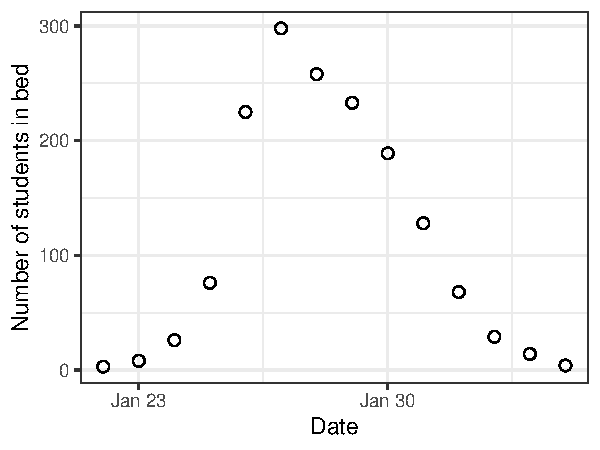
\includegraphics[width=.55\linewidth]{boarding_school/inbed.pdf}
		\end{figure}
	\end{itemize}	
}

\frame{
	\frametitle{Fitting a simple SIR}
	Specifying the model:
	\begin{itemize}
		\item prevalence data: $\mathds{I}_{t}$ with $t \in \{1,\ldots,14\}$
		\item parameters to estimate: $\theta = \{\beta,\gamma,\phi\}$
		\item parameters that will remain fixed: $\{S_0=762,I_0=1,R_0=0\}$
		\item map data $\mathds{I}_{t}$ to SIR model output $I(t)$ using an observation model  with an appropriate \alert{probability distribution}:
		$$
		\Pr(\mathds{I}|\theta) = \prod_{t=1}^{14} \text{neg-bin}(\mathds{I}_{t} | I(t), \phi)
		$$
		\item \alert{prior distributions} 
		\vspace{-1em}
		
		$$\Pr(\beta) = \text{exponential}(1)$$
		$$\Pr(1/\gamma) = \text{normal}(2,0.5)$$
		$$\Pr(1/\phi) = \text{exponential}(5)$$
	\end{itemize}
}

\frame{
	\frametitle{Fitting a simple SIR}
	We define the ODE system in the \texttt{function} block
		\begin{figure}
			\centering
			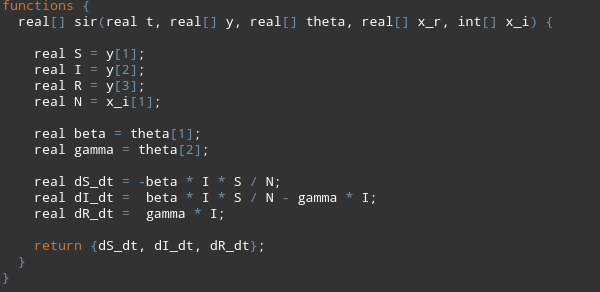
\includegraphics[width=1\linewidth]{boarding_school/stan_code1.png}
		\end{figure}
	\faWarning\ Be careful of the signature and formats!
}

\frame{
	\frametitle{Fitting a simple SIR}
	We declare the data variables in the \texttt{data} block
		\begin{figure}
			\centering
			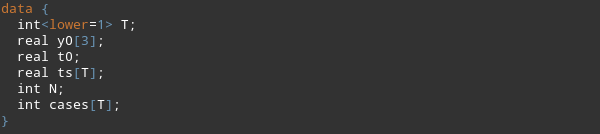
\includegraphics[width=1\linewidth]{boarding_school/stan_code2.png}
		\end{figure}
	
	\pause
	and define additional data variables in \texttt{transformed data}
	\begin{figure}
		\centering
		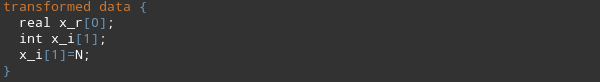
\includegraphics[width=1\linewidth]{boarding_school/stan_code3.png}
	\end{figure}
}

\frame{
	\frametitle{Fitting a simple SIR}
	Similarly, parameters are declared in the \texttt{parameters} block
		\begin{figure}
			\centering
			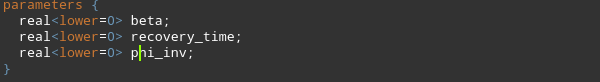
\includegraphics[width=1\linewidth]{boarding_school/stan_code4.png}
		\end{figure}
	\faWarning\ It sometimes makes more sense to transform some parameters (e.g., recovery rate $\gamma$ and overdispersion $\phi$) to improve interpretability
	}

\frame{
	\frametitle{Fitting a simple SIR}
	In \texttt{transformed parameters}, we define additional parameters and solve the ODE system
		\begin{figure}
			\centering
			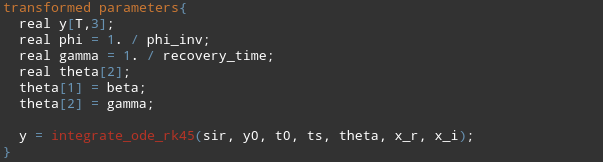
\includegraphics[width=1\linewidth]{boarding_school/stan_code5.png}
		\end{figure}
}


\frame{
	\frametitle{Fitting a simple SIR}
	\begin{figure}
		\centering
		
\includegraphics[width=.8\linewidth]{boarding_school/stan_code5bis.png}
	\end{figure}
	Two crucial points:
	\begin{itemize}
	\item be careful about the \alert{formats and signatures}
	\begin{itemize}
			\item[-] the ODE output \texttt{y} is an array of size \texttt{T}$\times$3 (number of time steps and number of compartments)
			\item[-] \texttt{sir} is the name of the function defined in the \texttt{function} block
			\item[-] \texttt{y0} is an array of size 3 defined in the \texttt{data} block
			\item[-] \texttt{ts} is an array of size \texttt{T} defined in the \texttt{data} block
			\item[-] \texttt{theta} is an array of size 2 storing the parameters
			\item[-] \texttt{x\_r} is defined as empty in \texttt{transformed data}, but can be used to store fixed real values
			\item[-] \texttt{x\_i} is an array of size 1 storing the population size \texttt{N} (can also be used to store fixed integer values)
	\end{itemize}
	\end{itemize}
}
\frame{
	\frametitle{Fitting a simple SIR}
	\begin{figure}
		\centering
		
\includegraphics[width=.8\linewidth]{boarding_school/stan_code5bis.png}
	\end{figure}
	Two crucial points:
	\begin{itemize}
		\item two ODE solvers are available:
	\begin{itemize}
		\item[-] \texttt{integrate\_ode\_rk45} uses the Runge-Kutta method (quicker but non-adapted to stiff systems)
		\item[-] \texttt{integrate\_ode\_bdf} uses the backward differentiation method (slower but adapted to stiff systems)
	\end{itemize}
	\end{itemize}
}

\frame{
	\frametitle{Fitting a simple SIR}
	In the \texttt{model} block, we write the priors and the observation model
	\begin{figure}
		\centering
		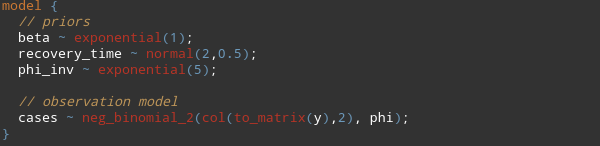
\includegraphics[width=1\linewidth]{boarding_school/stan_code6.png}
	\end{figure}
	\faWarning\ It's important that the chosen distributions correspond with the boundaries set in the \texttt{parameters} block (\texttt{<lower=0>})

\bigskip
	\faWarning\ \texttt{col(to\_to\_matrix(y))} extracts the 2nd column of \texttt{y}
}


\frame{
	\frametitle{Fitting a simple SIR}
	Last, we add a \texttt{generated quantities} block that does not influence sampling and can be used for ``post-processing'':
	\begin{itemize}
		\item reproduction number $\mathcal{R}_0 = \beta/\gamma$
		\item model predictions of prevalence from the negative binomial
	\end{itemize}

	\begin{figure}
		\centering
		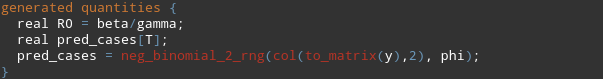
\includegraphics[width=1\linewidth]{boarding_school/stan_code7.png}
	\end{figure}
}

\frame{
	\frametitle{Fitting a simple SIR}
	In summary:
	\begin{itemize}
		\item \texttt{functions}: define the ODE system (\faWarning\ signature and formats)
		\item \texttt{data}: declare data variables that will be provided
		\item \texttt{tranformed data}: additional quantities that can be computed internally or from \texttt{data} variables 
		\item \texttt{parameters}: declare parameters (\faWarning\ boundaries)
		\item \texttt{transformed parameters}: quantities that can be computed internally or from \texttt{data} or \texttt{parameters} variables,
		including the ODE output (\faWarning \ signature and format)
		\item \texttt{model}: priors and observation model
		\item \texttt{generated quantities}: additional quantities that can be computed without influencing the sampling
	\end{itemize}

}


\frame{
	\frametitle{Fitting a simple SIR}
	As before, we conduct the inference from \texttt{R} with the package \texttt{rstan}:
	\begin{figure}
		\centering
		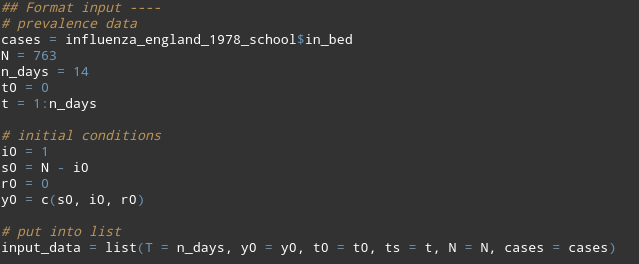
\includegraphics[width=1\linewidth]{boarding_school/r_code1.png}
	\end{figure}

	\faWarning\ data is put in a list with names matching the \texttt{data} block in Stan
}

\frame{
	\frametitle{Fitting a simple SIR}
	Hit the inference button!
	\begin{figure}
		\centering
		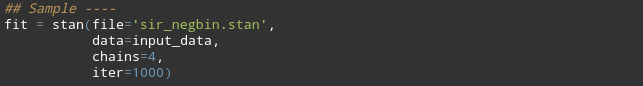
\includegraphics[width=1\linewidth]{boarding_school/r_code2.png}
	\end{figure}
}

\frame{
	\frametitle{Fitting a simple SIR}
	Run basic diagnosis tools:
	\begin{figure}
		\centering
		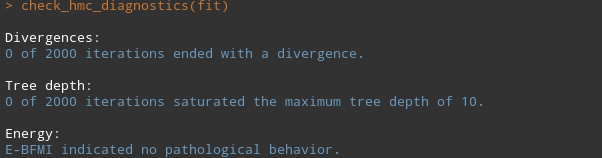
\includegraphics[width=1\linewidth]{boarding_school/r_code3.png}
	\end{figure}
}

\frame{
	\frametitle{Fitting a simple SIR}
	Examine trace plots:
	\begin{figure}
		\centering
		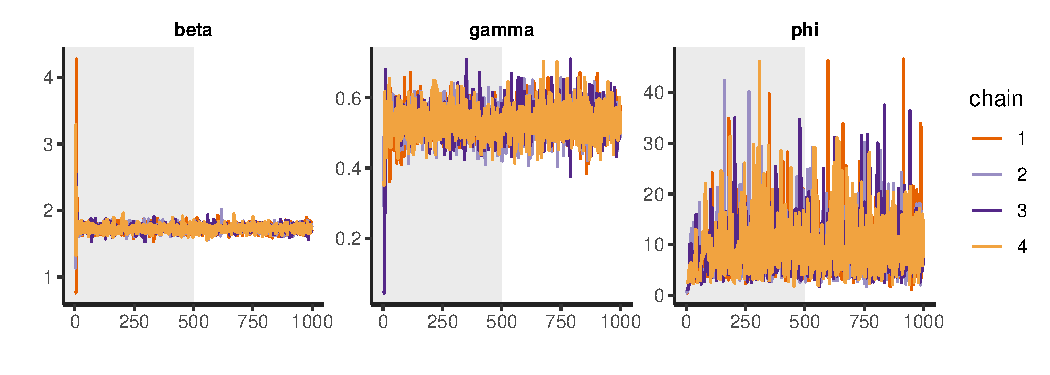
\includegraphics[width=1\linewidth]{boarding_school/trace_theta.pdf}
	\end{figure}
}

\frame{
	\frametitle{Fitting a simple SIR}
	Examine chain mixing:
	\begin{figure}
		\centering
		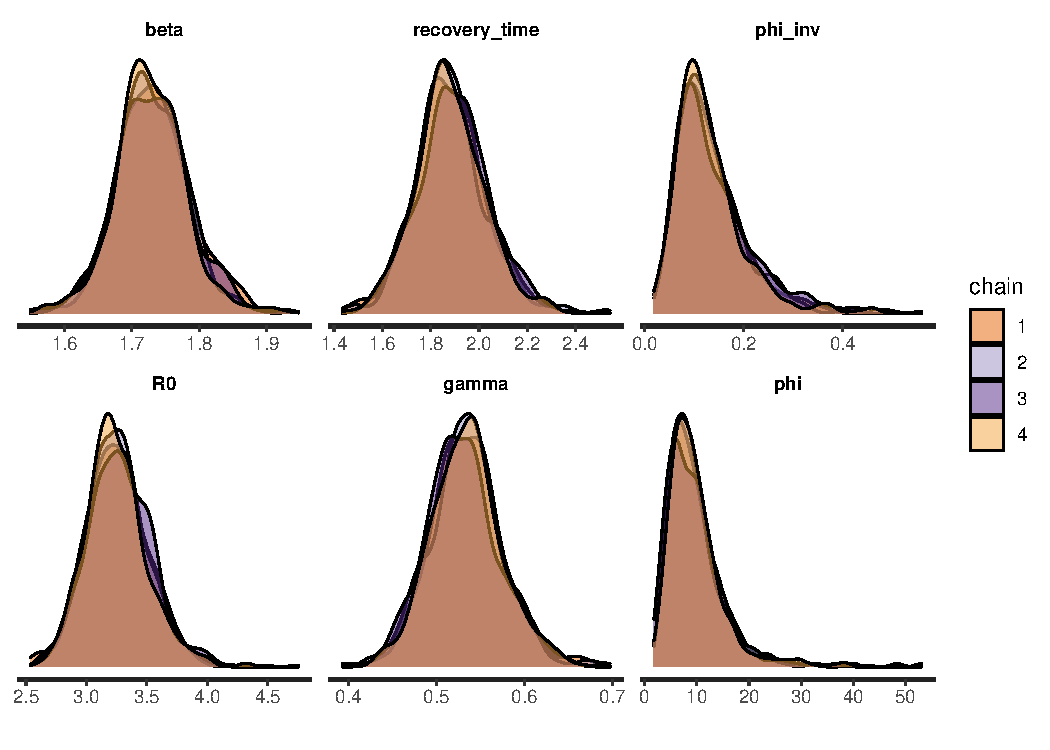
\includegraphics[width=.8\linewidth]{boarding_school/post_theta.pdf}
	\end{figure}
}

\frame{
	\frametitle{Fitting a simple SIR}
	Posterior predictive checking:
	\begin{figure}
		\centering
		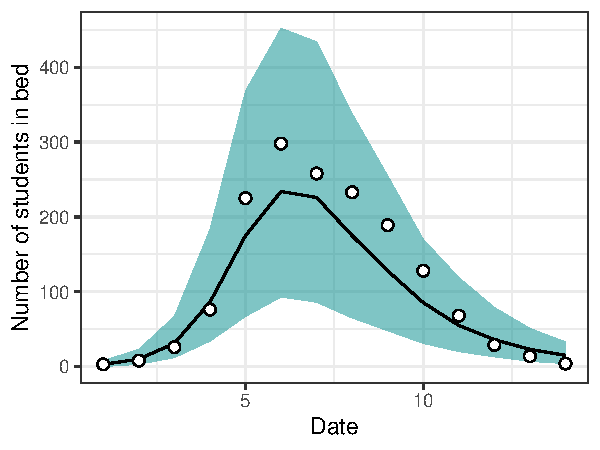
\includegraphics[width=.6\linewidth]{boarding_school/inbed_fit.pdf}
	\end{figure}
}

\frame{
	\frametitle{Fitting a simple SIR}
	Print the results:
	\begin{figure}
		\centering
		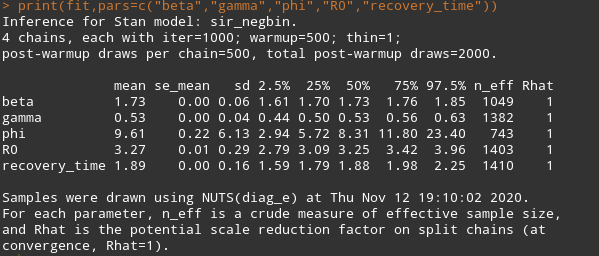
\includegraphics[width=1\linewidth]{boarding_school/r_code4.png}
	\end{figure}
}

\frame{
	\frametitle{Fitting a simple SIR}
	Conclusions:
	\begin{itemize}
		\item we estimate $\mathcal{R}_0$ to 3.3 (95\% credible interval: 2.8 to 4.0)
		\item this corresponds to the direct estimation from the final size of the epidemic $q = 512/763 = 0.67$
		\vspace{-.5em}
		$$
		\mathcal{R}_0 = 1 / (1-q) = 3.03
		$$
		\item based on \alert{many assumptions}:
		\begin{itemize}
			\item[-] common to all SIRs (homogeneous mixing, no incubation...)
			\item[-] prior distributions (especially on the recovery period)
			\item[-] complete ascertainment, no asymptomatics
			\item[-] no initial immunity
		\end{itemize}
	\end{itemize}
		
}

\frame{
	\frametitle{Outline}
	\begin{itemize}
		\item Introduction
		\item (Quick notice: Bayesian inference with Stan)
		\item Fitting a simple SIR
		\item \textbf{Simulations to understand the model}
		\item Scaling up ODE-based models
		\item Extensions 
	\end{itemize}
}

\frame{
	\frametitle{Simulations to understand the model}
	In practice, the situation is often less clear than in the boarding school example:
	\begin{itemize}
		\item[-] incomplete data, insufficient domain knowledge
		\item[-] uncertainty on \alert{necessary model features}
	\end{itemize}
	\alert{Fake data} can be used to probe the model and better understand its behaviour:
	\begin{itemize}
		\item[-] prior predictive checking
		\item[-] model reliability checking
	\end{itemize}	
}

\frame{
	\frametitle{Simulations to understand the model}
	\alert{Prior predictive checking} consists in simulating data from the priors:
	\begin{itemize}
		\item visualize priors (especially after transformation)
		\item this shows the range of data compatible with the model
		\item it helps understand the \alert{adequacy of the chosen priors}, as it is often easier to elicit expert knowledge on measureable quantities of interest rather than abstract parameter values
		\bigskip\pause
		\item remove (or switch off) the likelihood from the \texttt{model} block
	\end{itemize}
	\begin{figure}
		\centering
		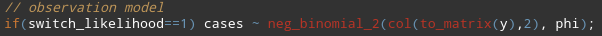
\includegraphics[width=1\linewidth]{boarding_school/stan_code6bis.png}
	\end{figure}
}

\frame{
	\frametitle{Simulations to understand the model}
	Simulating priors in the boarding school example:
	\begin{figure}
		\centering
		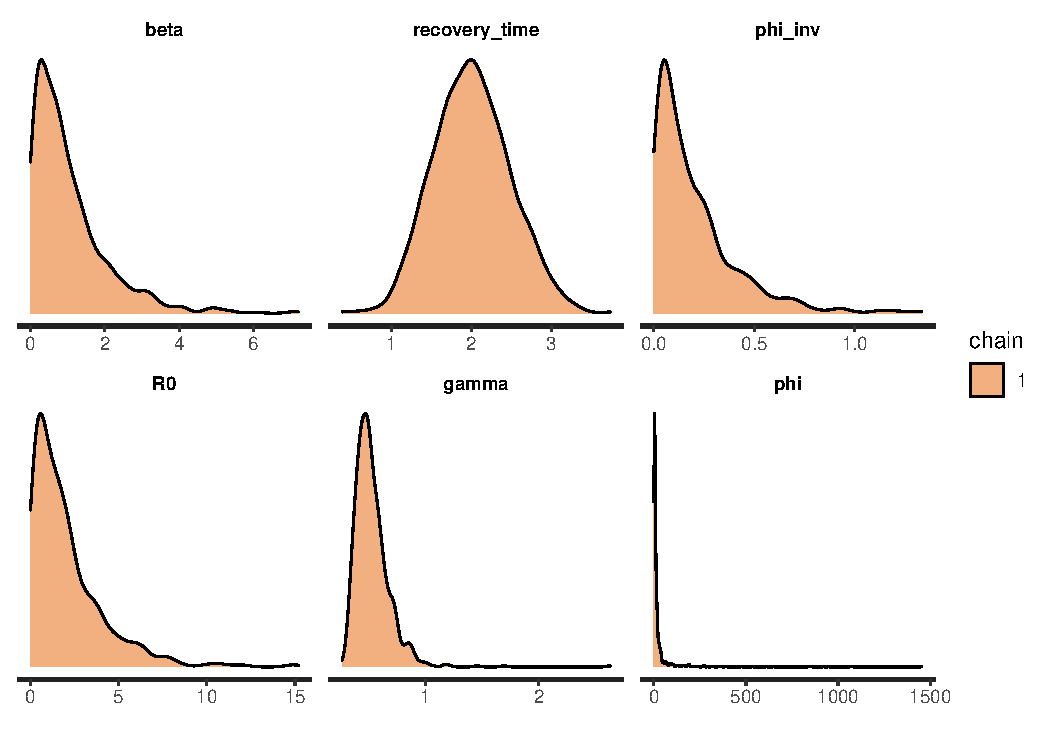
\includegraphics[width=.8\linewidth]{boarding_school/prior_theta.pdf}
	\end{figure}
}

\frame{
	\frametitle{Simulations to understand the model}
	Prior predictive checking: simulating \alert{epidemic trajectories}
	\begin{figure}
		\centering
		\only<1>{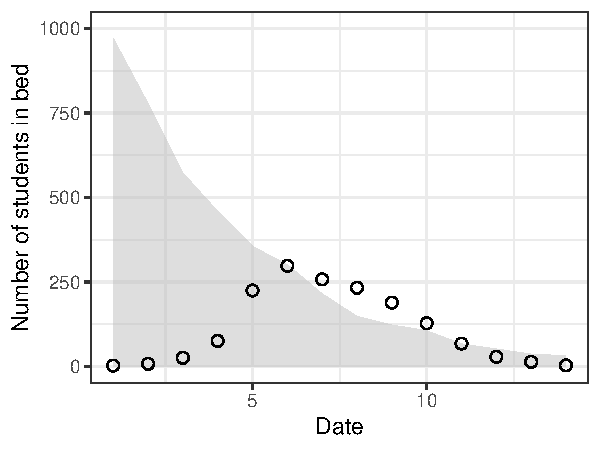
\includegraphics[width=.6\linewidth]{boarding_school/inbed_fit_prior.pdf}}
		\only<2>{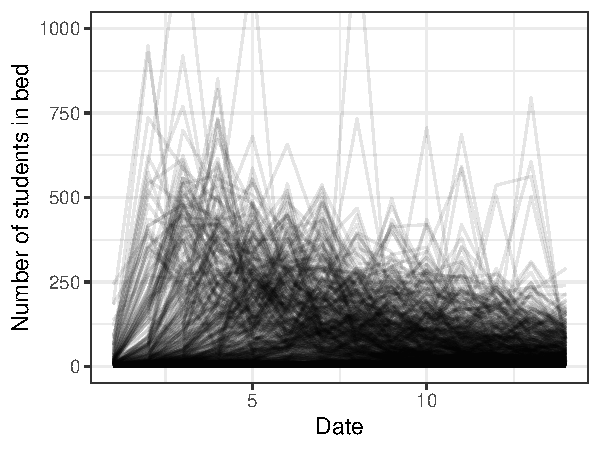
\includegraphics[width=.6\linewidth]{boarding_school/inbed_fit_prior_traj.pdf}}
	\end{figure}
}

\frame{
	\frametitle{Simulations to understand the model}
	Prior predictive checking brings insight about \alert{non-obvious features}:
	\begin{itemize}
		\item while the priors seem large and weakly informative, there is actually not a lot of leeway
		\item \alert{highly constrained} model: 
		\begin{itemize}
		\item[-] if $\beta$ is high, the epidemic will stop rapidly by lack of susceptibles
		\item[-] if $\beta$ is small, the epidemic will be small
	\end{itemize}
	\item the negative binomial might lead to problems in extreme situations, e.g. more cases (>1000) than the overall number of students
	\end{itemize}
}

\frame{
	\frametitle{Simulations to understand the model}
	\alert{Model reliability checking} consists in attempting to recover chosen parameter values with the model:
	identifiability issues
	
}


\frame{
	\frametitle{Acknowledgements \& ressources}
	\begin{itemize}
		\item Michael Betancourt, \textit{Introduction to Stan} \\ \url{https://betanalpha.github.io/assets/case_studies/stan_intro.html}
		\item Andrew Gelman et al., \textit{Bayesian workflow} \\ \url{https://arxiv.org/abs/2011.01808}
		\item Daniel Lee, \textit{ODEs in Stan} \\ \url{https://youtu.be/hJ34_xJhYeY}
		\item Richard McElreath, \textit{Statistical rethinking} \url{https://youtu.be/4WVelCswXo4}
	
	\end{itemize}
}


\end{document}
